\chapter{Sau Hartree--Fock: CI, MP2 và Coupled Cluster}
\label{ch:sauhf}

Hartree--Fock cho ta một định thức Slater tốt nhất. Các phương pháp ``sau Hartree--Fock'' \en{post-Hartree--Fock} đi tiếp từ đó và cố gắng thu lại năng lượng tương quan còn thiếu. Chương này trình bày ba ý tưởng chính: trộn thêm nhiều định thức (CI), coi tương quan như một nhiễu loạn nhỏ (MP2), và ``lãi kép'' các kích thích (Coupled Cluster).

\section{Tương tác cấu hình (CI): pha màu}

\begin{eli5}[pha màu]
Màu thật (hàm sóng đúng) được pha từ một màu nền (định thức HF) với một chút các màu khác. Mỗi ``màu khác'' là một \textbf{định thức kích thích} \en{excited determinant}: lấy 1, 2 hoặc 3 electron từ orbital đang có người lên các orbital còn trống (orbital ``ảo'' \en{virtual}). Dùng \emph{tất cả} các màu trong hộp gọi là \textbf{Full CI}: chính xác tuyệt đối \emph{với hộp màu đó} (tức là với tập cơ sở đã chọn). Hộp càng nhiều màu (tập cơ sở lớn) thì càng gần màu thật.

\emph{Chỗ ví dụ ``gãy'':} hệ số pha có thể âm (các định thức giao thoa triệt tiêu nhau), điều không xảy ra với sơn. Và số ``màu'' tăng nhanh khủng khiếp.
\end{eli5}

\begin{congthuc}[khai triển CI]
\[
|\Psi_{\rm CI}\rangle=c_0|\Phi_0\rangle+\sum_{a,r}c_a^r|\Phi_a^r\rangle+\sum_{\substack{a<b\\ r<s}}c_{ab}^{rs}|\Phi_{ab}^{rs}\rangle+\sum_{\substack{a<b<c\\ r<s<t}}c_{abc}^{rst}|\Phi_{abc}^{rst}\rangle+\cdots
\]
\begin{itemize}
\item $\Phi_0$: định thức HF. $\Phi_a^r$: định thức trong đó electron ở orbital chiếm $a$ được chuyển lên orbital ảo $r$ (kích thích đơn). $\Phi_{ab}^{rs}$: kích thích đôi, v.v.
\item Các hệ số $c$ tìm bằng cách chéo hóa ma trận $H_{IJ}=\langle\Phi_I|\Hhat|\Phi_J\rangle$. Trị riêng nhỏ nhất là năng lượng. Đây là phương pháp biến phân nên cho cận trên.
\item Cắt bớt theo bậc kích thích: CIS (đơn), CISD (đơn + đôi), CISDT\ldots{} Giữ tất cả là \textbf{Full CI} (FCI).
\item \textbf{Định lý Brillouin}: với định thức HF, $\langle\Phi_0|\Hhat|\Phi_a^r\rangle=0$. Kích thích đơn không trực tiếp hạ năng lượng; tương quan bắt đầu từ kích thích đôi, tức là \emph{từng cặp} electron cùng né nhau.
\end{itemize}
Với Li chỉ có 3 electron, bậc kích thích cao nhất là 3, nên CISDT đã là Full CI.
\end{congthuc}

\subsection{Bùng nổ tổ hợp}
Có bao nhiêu định thức? Với $M$ orbital không gian, $N_\alpha$ electron spin lên và $N_\beta$ electron spin xuống, số cách chọn là
\[
N_{\rm det}=\binom{M}{N_\alpha}\binom{M}{N_\beta}.
\]
Với Li ($N_\alpha=2,N_\beta=1$) trong tập cc-pCVQZ ($M=84$): $\binom{84}{2}\times84=3486\times84=292\,824$ định thức, một con số máy tính xách tay xử lý trong vài phút. Nhưng hình~\ref{fig:dinhthuc} cho thấy chuyện gì xảy ra khi số electron tăng: với Ne (10 electron) và 100 orbital đã có $\sim10^{15}$ định thức, còn với Fe là $\sim10^{31}$. Đây chính là bức tường hàm mũ của chương~\ref{ch:baitoan}, trong một bộ áo khác. Năm 2017, một nhóm nghiên cứu đã chạy được một vòng lặp CI với khoảng $10^{12}$ định thức trên siêu máy tính \cite{Vogiatzis2017}, cỡ giới hạn của công nghệ hiện nay.

\begin{figure}[h]
\centering
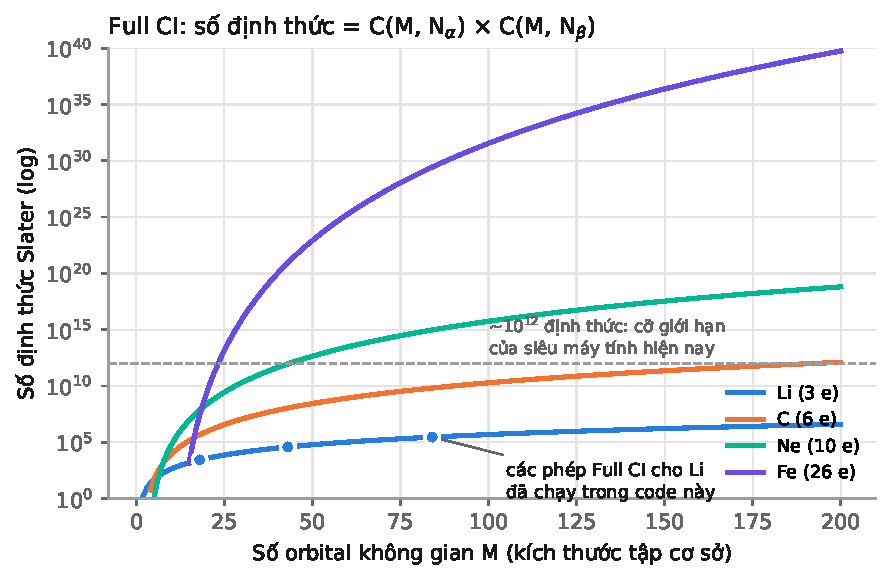
\includegraphics[width=0.84\textwidth]{03_bung_no_dinh_thuc.pdf}
\caption{Số định thức của Full CI theo số orbital, cho các nguyên tử có số electron khác nhau (trục tung thang log). Các chấm xanh là ba phép Full CI cho Li chạy trong code đi kèm. (Script \code{03\_sau\_hartree\_fock.py})}
\label{fig:dinhthuc}
\end{figure}

\subsection{Vấn đề ``nhất quán kích thước''}
CI cắt bớt (như CISD) có một khuyết tật tinh tế. Xét hai nguyên tử Li đặt cách nhau 50\,Å, xa tới mức không tương tác. Năng lượng của cặp phải đúng bằng hai lần năng lượng một nguyên tử. Nhưng hàm sóng đúng của cặp chứa số hạng ``kích thích đôi trên nguyên tử A \emph{nhân} kích thích đôi trên nguyên tử B'', tức là kích thích bậc 4 của cả hệ, mà CISD không có. Subagent nghiên cứu đã kiểm tra trực tiếp bằng PySCF (tập cc-pCVDZ): CISD cho năng lượng cặp cao hơn hai lần năng lượng một nguyên tử $0.19\mHa$, trong khi MP2 và CCSD cho đúng sai lệch bằng 0. Tính chất ``năng lượng của các mảnh không tương tác thì cộng được'' gọi là \textbf{nhất quán kích thước} \en{size-consistency}. Với hệ lớn, sai số của CISD tăng như $\sqrt{N}$ thay vì $N$, và tỉ lệ tương quan thu được trên mỗi phân tử tiến về 0 \cite{Szabo1996}. Đó là lý do CISD hầu như không còn được dùng.

\section{Lý thuyết nhiễu loạn Møller--Plesset (MP2)}

\begin{eli5}[giá khởi điểm và phụ phí]
Lấy năng lượng HF làm ``giá khởi điểm'', rồi cộng thêm một khoản ``phụ phí'' cho từng cặp electron, tính xem chúng muốn né nhau bao nhiêu. Phụ phí bậc 2 thường là phần lớn nhất. Nhanh, rẻ, nhưng nếu giá khởi điểm tệ (khi HF là bức tranh sai về chất) thì phụ phí có thể không còn ``nhỏ''.
\end{eli5}

\begin{congthuc}[MP2]
Coi Hamiltonian là tổng các toán tử Fock (bài toán đã giải được) cộng một nhiễu loạn $\hat V$. Bổ chính bậc 2 \cite{MollerPlesset1934}:
\[
E^{(2)}=\frac14\sum_{a,b}^{\text{chiếm}}\sum_{r,s}^{\text{ảo}}\frac{|\langle ab\|rs\rangle|^2}{\varepsilon_a+\varepsilon_b-\varepsilon_r-\varepsilon_s}\;<0 .
\]
\begin{itemize}
\item $\langle ab\|rs\rangle$: ``độ mạnh'' của việc đẩy cặp electron từ orbital $a,b$ lên $r,s$ (tích phân đẩy đã phản đối xứng hóa).
\item Mẫu số: chênh lệch năng lượng orbital, luôn âm. Kích thích càng ``đắt'' thì đóng góp càng nhỏ.
\end{itemize}
MP2 không cần lặp, chi phí tăng như $N^5$, nhất quán kích thước, nhưng \emph{không biến phân}: có thể cho năng lượng thấp hơn giá trị đúng.
\end{congthuc}

\section{Coupled Cluster: lãi kép thay vì lãi đơn}

\begin{eli5}[lãi kép]
CI cộng mỗi kích thích đúng một lần, giống ``lãi đơn''. Coupled Cluster đặt các kích thích vào \emph{số mũ}, giống ``lãi kép'': $e^{\hat T}=1+\hat T+\tfrac12\hat T^2+\tfrac16\hat T^3+\ldots$ Nhờ vậy nó tự động sinh ra mọi tổ hợp của các kích thích độc lập, ví dụ ``cặp này né nhau \emph{và đồng thời} cặp kia né nhau''. Hai phân tử ở xa nhau được mô tả đúng như hai hệ riêng biệt, tức là nhất quán kích thước.

\emph{Chỗ ví dụ ``gãy'':} CC không biến phân. Và nếu ``vốn ban đầu'' (định thức HF) sai về bản chất (khi cần nhiều định thức ngang nhau), thì lãi kép từ một số vốn sai vẫn sai.
\end{eli5}

\begin{congthuc}[Coupled Cluster]
\[
|\Psi_{\rm CC}\rangle=e^{\hat T}|\Phi_0\rangle,\qquad \hat T=\hat T_1+\hat T_2+\hat T_3+\ldots
\]
\begin{itemize}
\item $\hat T_1=\sum_{ar}t_a^r\,\hat a_r^\dagger\hat a_a$ tạo kích thích đơn với ``biên độ'' $t_a^r$; $\hat T_2=\tfrac14\sum t_{ab}^{rs}\hat a_r^\dagger\hat a_s^\dagger\hat a_b\hat a_a$ tạo kích thích đôi. ($\hat a^\dagger$, $\hat a$: toán tử ``đặt'' và ``nhấc'' một electron.)
\item Khai triển $e^{\hat T_2}=1+\hat T_2+\tfrac12\hat T_2^2+\ldots$: số hạng $\tfrac12\hat T_2^2$ là kích thích bậc 4 dạng ``đôi nhân đôi''. Đây đúng là thứ CISD thiếu.
\item Các biên độ $t$ được tìm bằng cách giải hệ phương trình phi tuyến (lặp). \textbf{CCSD} giữ $\hat T_1+\hat T_2$ \cite{PurvisBartlett1982}, chi phí $\sim N^6$.
\item \textbf{CCSD(T)} thêm ước lượng nhiễu loạn cho kích thích ba, chi phí $\sim N^7$ \cite{Raghavachari1989}. Đây được gọi là ``tiêu chuẩn vàng'' \en{gold standard} của hóa lượng tử cho các phân tử có một cấu hình chiếm ưu thế \cite{BartlettMusial2007}.
\end{itemize}
\end{congthuc}

\begin{table}[h]
\centering\small
\caption{Thứ bậc các phương pháp hàm sóng. $N$ là kích thước hệ (số electron hoặc số hàm cơ sở) \cite{BartlettMusial2007,Szabo1996}.}
\label{tab:chiphi}
\begin{tabular}{@{}llccl@{}}
\toprule
Phương pháp & Chi phí & Biến phân? & Nhất quán kích thước? & Ghi chú \\
\midrule
HF & $N^4$ & có & có & không có tương quan \\
MP2 & $N^5$ & không & có & rẻ, thường thu 80--95\% tương quan \\
CISD & $N^6$ & có & \textbf{không} & ít dùng vì lỗi kích thước \\
CCSD & $N^6$ & không & có & lặp \\
CCSD(T) & $N^7$ & không & có & ``tiêu chuẩn vàng'' \\
Full CI & tổ hợp ($\sim e^N$) & có & có & chính xác trong tập cơ sở \\
\bottomrule
\end{tabular}
\end{table}

\begin{figure}[h]
\centering
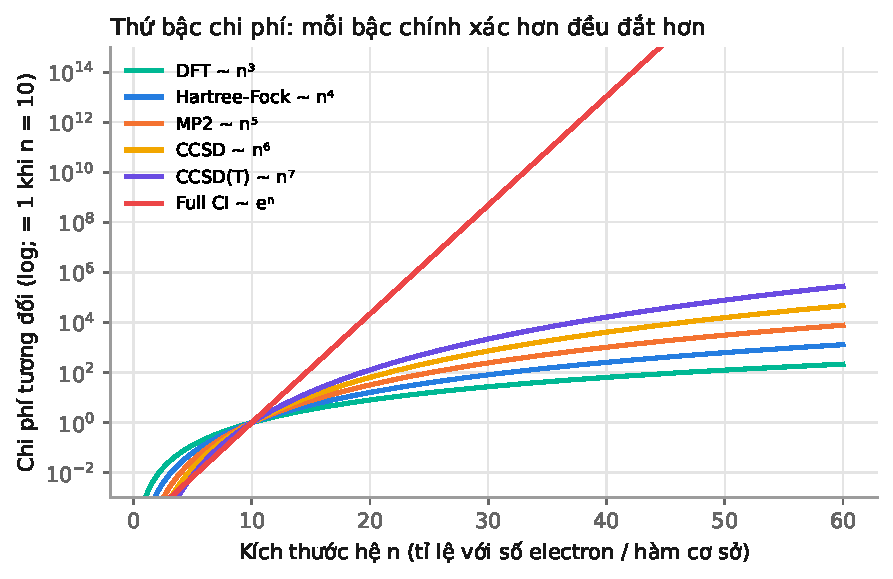
\includegraphics[width=0.8\textwidth]{03_chi_phi.pdf}
\caption{Chi phí tương đối theo kích thước hệ. Tăng kích thước 2 lần thì HF đắt hơn 16 lần, CCSD(T) đắt hơn 128 lần, còn Full CI thì tăng theo hàm mũ. (Minh họa theo bậc lý thuyết, script \code{03\_sau\_hartree\_fock.py})}
\label{fig:chiphi}
\end{figure}

\section{Kết quả cho Li}\label{sec:ketquasauhf}

\begin{chaycode}[chạy mọi phương pháp trên Li]
Script \code{03\_sau\_hartree\_fock.py} chạy UHF, MP2, CISD, CCSD, CCSD(T) và Full CI cho Li với ba tập cơ sở lõi--hóa trị cc-pCVDZ, cc-pCVTZ, cc-pCVQZ (18, 43, 84 hàm), đo thời gian chạy, rồi ngoại suy về tập cơ sở vô hạn. Cả 6 phương pháp chạy hết trong vài phút trên máy tính xách tay.
\end{chaycode}

\begin{table}[h]
\centering\small
\caption{Năng lượng của Li (Ha) tính bằng code đi kèm. Trong ngoặc: sai số so với năng lượng chính xác (mHa). Dòng cuối: phần trăm năng lượng tương quan thu được ở cc-pCVQZ. Cột CBS: HF giới hạn cộng năng lượng tương quan ngoại suy từ T và Q.}
\label{tab:sauhf}
\begin{tabular}{@{}lllll@{}}
\toprule
Phương pháp & cc-pCVDZ & cc-pCVTZ & cc-pCVQZ & CBS (T,Q) \\
\midrule
UHF & $-7.43244$ (45.62) & $-7.43270$ (45.36) & $-7.43272$ (45.34) & --- \\
MP2 & $-7.46145$ (16.61) & $-7.46987$ (8.19) & $-7.47227$ (5.79) & $-7.47401$ (4.05) \\
CISD & $-7.46602$ (12.04) & $-7.47422$ (3.84) & $-7.47633$ (1.73) & --- \\
CCSD & $-7.46602$ (12.04) & $-7.47423$ (3.83) & $-7.47633$ (1.73) & $-7.47787$ (0.19) \\
CCSD(T) & $-7.46602$ (12.04) & $-7.47425$ (3.81) & $-7.47637$ (1.69) & $-7.47791$ (0.15) \\
FCI & $-7.46603$ (12.04) & $-7.47425$ (3.81) & $-7.47637$ (1.69) & $-7.47794$ (0.12) \\
\midrule
Số hàm cơ sở & 18 & 43 & 84 & $\infty$ \\
Số định thức FCI & 2\,754 & 38\,829 & 292\,824 & --- \\
\% tương quan (QZ) & \multicolumn{4}{l}{MP2 87.2\%, CISD 96.2\%, CCSD 96.2\%, CCSD(T) 96.3\%, FCI 96.3\%} \\
\bottomrule
\end{tabular}
\end{table}


Bảng~\ref{tab:sauhf} và hình~\ref{fig:tuongquan} cho ba bài học quan trọng.

\paragraph{Bài học 1: với Li, tập cơ sở quan trọng hơn phương pháp.} Trong cùng một tập cơ sở, CISD, CCSD, CCSD(T) và FCI gần như trùng nhau (chênh nhau dưới $0.1\mHa$), vì với 3 electron, phần thiếu của CISD hay CCSD chỉ là kích thích ba, mà phần này rất nhỏ. MP2 thiếu khoảng 10\% (ở cc-pCVQZ, MP2 thu \PctMPtwoQZ\% năng lượng tương quan đúng). Nhưng cùng một phương pháp FCI, đổi từ cc-pCVDZ sang cc-pCVQZ làm năng lượng thay đổi tới $10\mHa$. Sai số còn lại của FCI/cc-pCVQZ ($\ErrFciQZ\mHa$) hoàn toàn do tập cơ sở chưa đủ lớn.

\paragraph{Bài học 2: năng lượng tương quan hội tụ chậm, nhưng ngoại suy được.} Lý thuyết (gắn với mũi nhọn Kato, mục~\ref{sec:cusp}) cho biết sai số tương quan giảm như $X^{-3}$, với $X$ là ``bậc'' tập cơ sở \cite{Helgaker1997}. Từ hai giá trị ở $X=3$ (T) và $X=4$ (Q) có thể ngoại suy về tập cơ sở vô hạn:
\[
E_{\rm corr}(\infty)\approx\frac{4^3E_{\rm corr}(4)-3^3E_{\rm corr}(3)}{4^3-3^3}.
\]
Ngoại suy FCI theo cách này thu được \PctFciCBS\% năng lượng tương quan đúng của Li, sai số chỉ còn $\ErrFciCBS\mHa$, tốt hơn độ chính xác hóa học hơn 10 lần.

\begin{figure}[h]
\centering
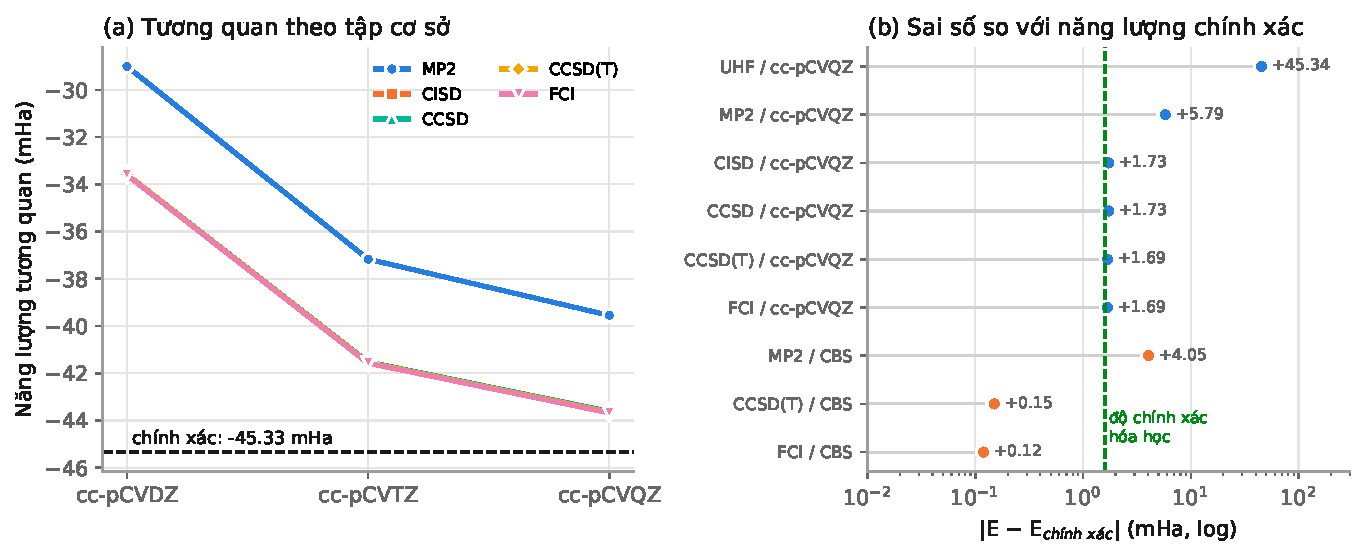
\includegraphics[width=\textwidth]{03_tuong_quan_theo_tap_co_so.pdf}
\caption{(a) Năng lượng tương quan thu được theo tập cơ sở: mọi phương pháp tương quan đầy đủ gần như trùng nhau, MP2 thấp hơn một chút; tất cả đều tiến dần về giá trị đúng $-45.33\mHa$ nhưng chậm. (b) Sai số so với năng lượng chính xác (thang log). Ngoại suy CBS kéo sai số FCI xuống dưới độ chính xác hóa học (vạch xanh lá). (Script \code{03\_sau\_hartree\_fock.py})}
\label{fig:tuongquan}
\end{figure}

\paragraph{Bài học 3: phải có hàm ``lõi''.} Tương quan của Li nằm chủ yếu ở cặp 1s$^2$ (chương~\ref{ch:hatdongnhat}). Tập cc-pVXZ chuẩn được thiết kế cho electron hóa trị, hầu như không có hàm nào ``chạm'' tới vùng lõi. Kết quả trong bảng~\ref{tab:loi} khá sốc: FCI với cc-pVQZ (55 hàm) chỉ thu \PctCorePVQZ\% năng lượng tương quan, trong khi cc-pCVQZ thu \PctCoreCVQZ\%. \emph{Loại} hàm quan trọng hơn \emph{số lượng} hàm. Một lỗi thực hành nguy hiểm khác là ``đóng băng lõi'' \en{frozen core}, một tùy chọn mặc định ở nhiều chương trình. Với Li, đóng băng 1s$^2$ là xóa sạch gần như toàn bộ tương quan.

\begin{table}[h]
\centering\small
\caption{Full CI cho Li với hai tập cơ sở cỡ QZ: không có và có hàm lõi.}
\label{tab:loi}
\begin{tabular}{@{}lrrr@{}}
\toprule
Tập cơ sở & Số hàm & $\Ecorr$ (FCI, mHa) & \% của giá trị đúng \\
\midrule
cc-pVQZ & 55 & $-17.14$ & 37.8\% \\
cc-pCVQZ & 84 & $-43.68$ & 96.3\% \\
\midrule
Giá trị đúng & $\infty$ & $-45.33$ & 100\% \\
\bottomrule
\end{tabular}
\end{table}


\subsection{Hàm sóng Full CI trông như thế nào?}
Code cũng ``mổ xẻ'' hàm sóng FCI/cc-pCVQZ của Li. Định thức HF có hệ số $c_0$ với $c_0^2=\czeroSq$: hàm sóng thật gần như hoàn toàn là ``Hartree--Fock''. Tất cả hơn 290\,000 định thức còn lại chỉ chia nhau phần nhỏ còn lại (dưới 1\%), phần lớn là kích thích đôi của cặp 1s$^2$ lên các orbital ảo. Vậy là chưa tới 1\% ``trọng lượng'' hàm sóng gánh toàn bộ $45\mHa$ năng lượng tương quan. Li là một hệ \textbf{đơn tham chiếu} \en{single-reference} điển hình: một định thức chiếm ưu thế tuyệt đối, nên các phương pháp dựa trên HF (MP2, CC) hoạt động rất tốt.

\section{Khi một định thức không đủ: phương pháp đa tham chiếu}
Có những hệ mà định thức HF \emph{không} chiếm ưu thế, ví dụ khi bẻ gãy liên kết hóa học, ở nhiều hợp chất kim loại chuyển tiếp, hay ở nguyên tử Be (cấu hình 1s$^2$2p$^2$ trộn mạnh với 1s$^2$2s$^2$). Khi đó cần \textbf{phương pháp đa tham chiếu}, phổ biến nhất là CASSCF \cite{Roos1980}: chọn một ``không gian hoạt động'' gồm vài electron và vài orbital quan trọng, làm Full CI trong không gian nhỏ đó, đồng thời tối ưu luôn các orbital. Sau đó thường thêm tương quan động bằng nhiễu loạn (CASPT2) hoặc CI (MRCI). Li ở trạng thái cơ bản không cần những phương pháp này.

\section{Đưa thẳng $r_{12}$ vào hàm sóng}
Vì sao FCI với gần 300\,000 định thức vẫn sai $\ErrFciQZ\mHa$? Vì tổ hợp các orbital mượt rất khó tạo ra mũi nhọn $\Psi\approx\Psi(0)(1+\tfrac12r_{12})$. Năm 1929, Hylleraas đưa thẳng khoảng cách $r_{12}$ vào hàm thử cho He \cite{Hylleraas1929}. Với Li, hàm Hylleraas có dạng
\[
\phi=r_{23}^{n_1}r_{31}^{n_2}r_{12}^{n_3}\,r_1^{n_4}r_2^{n_5}r_3^{n_6}\,e^{-\alpha r_1-\beta r_2-\gamma r_3}\times(\text{hàm spin}).
\]
Hiệu quả rất lớn: 60 hàm Hylleraas (Larsson 1968) đã cho sai số $0.035\mHa$ \cite{Larsson1968}, nhỏ hơn 50 lần sai số của FCI với 292\,824 định thức Gauss. Với 34\,020 hàm, Wang và cộng sự (2012) đạt 15 chữ số \cite{Wang2012}. Cái giá phải trả là các tích phân 3 electron, 4 electron trở nên cực kỳ khó, nên phương pháp Hylleraas thuần chỉ dùng được cho hệ rất nhỏ.

Phiên bản ``thực dụng'' cho phân tử là các phương pháp \textbf{F12} (hay R12): giữ khung CI/CC thông thường nhưng thêm cho mỗi cặp electron một số hạng phụ thuộc $r_{12}$ \cite{Kutzelnigg1985,Hattig2012}. CCSD(T)-F12 với tập cơ sở cỡ TZ thường chính xác ngang CCSD(T) thông thường với tập 5Z, trong khi nhanh hơn khoảng 100 lần \cite{Adler2007}.

\begin{ghinho}
\begin{itemize}
\item CI trộn định thức HF với các định thức kích thích. Full CI chính xác \emph{trong tập cơ sở}, nhưng số định thức tăng theo tổ hợp: bức tường hàm mũ lại xuất hiện.
\item CI cắt bớt (CISD) không nhất quán kích thước. MP2 ($N^5$) và Coupled Cluster ($e^{\hat T}$, CCSD $N^6$, CCSD(T) $N^7$) nhất quán kích thước nhưng không biến phân.
\item Với Li, mọi phương pháp tương quan đầy đủ gần như trùng nhau; sai số chủ yếu do tập cơ sở. Cần hàm lõi (cc-pCVXZ); ngoại suy $X^{-3}$ đưa FCI về sai số $\sim0.1\mHa$.
\item Mũi nhọn Kato làm khai triển theo orbital hội tụ chậm. Đưa $r_{12}$ vào hàm sóng (Hylleraas, F12) khắc phục điều này.
\end{itemize}
\end{ghinho}
